\documentclass[tikz, border=12pt]{standalone}
\usepackage{tikz}
\usepackage{amsmath}
\usetikzlibrary{shapes.geometric, arrows.meta, positioning, shadows.blur, backgrounds, fit, calc}

\begin{document}

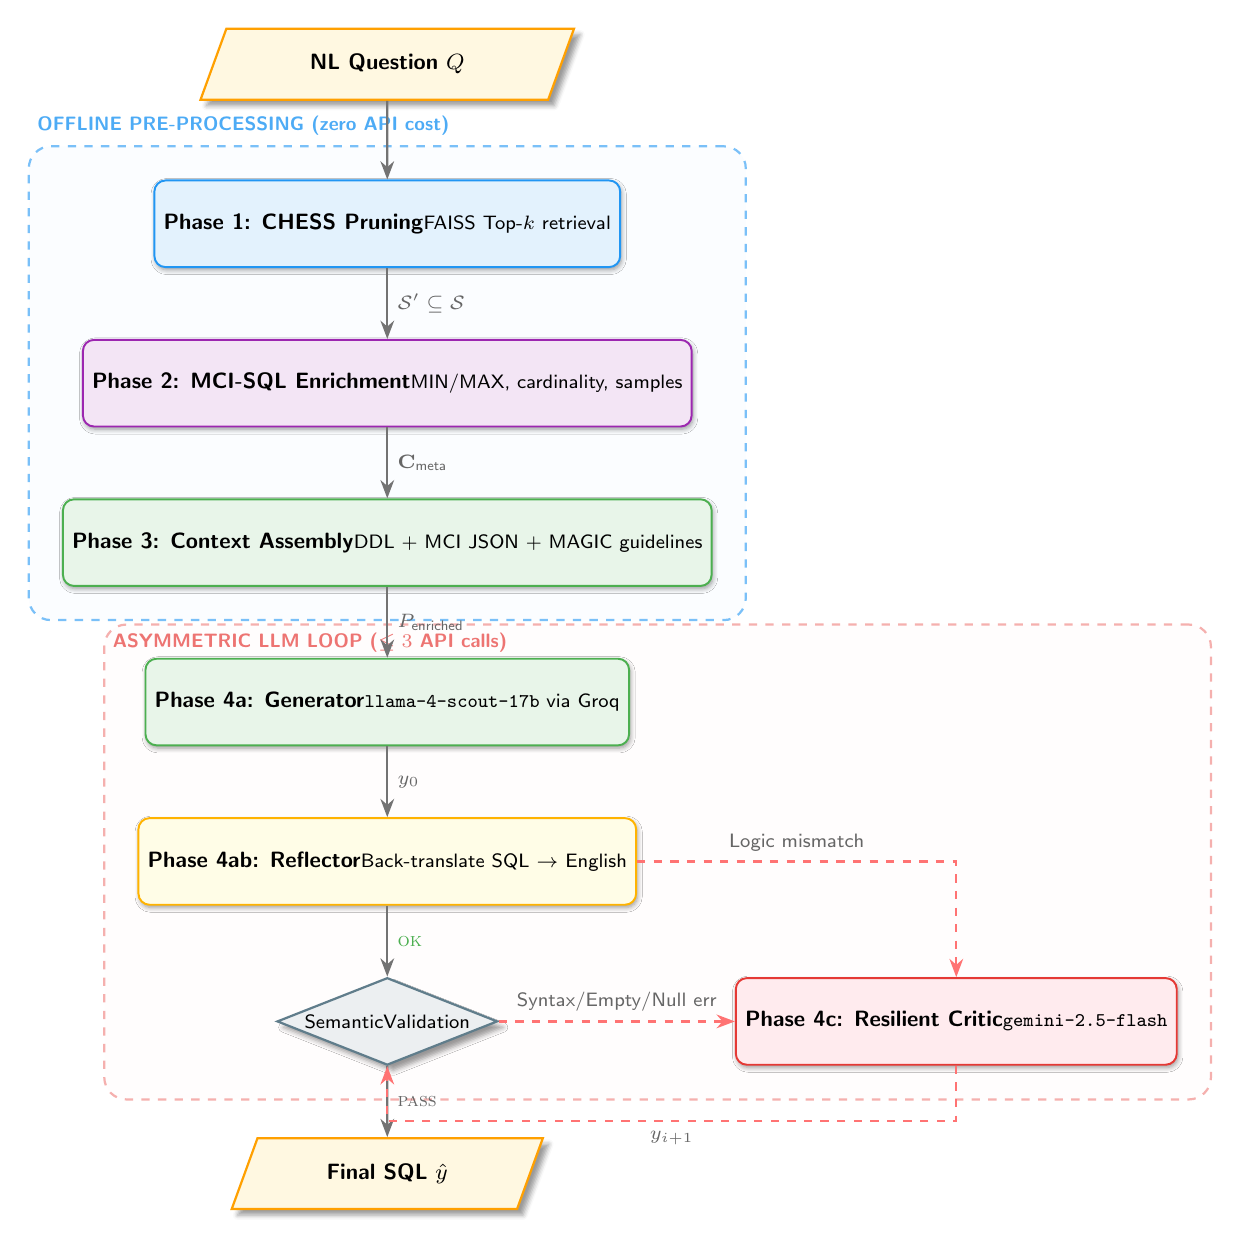
\begin{tikzpicture}[
    node distance=1.2cm and 2.5cm,
    font=\sffamily\footnotesize,
    >=Stealth,
    % --- Styles ---
    phase/.style={
        rectangle, minimum width=5.2cm, minimum height=1.1cm,
        text centered, rounded corners=4pt, line width=0.7pt,
        blur shadow={shadow blur steps=6, shadow xshift=0.5pt, shadow yshift=-1pt}
    },
    io/.style={
        trapezium, trapezium left angle=70, trapezium right angle=110,
        minimum width=3.5cm, minimum height=0.9cm,
        text centered, draw=io_border, fill=io_fill,
        line width=0.8pt, blur shadow={shadow blur steps=4}
    },
    decision/.style={
        diamond, aspect=2.5, minimum width=2.8cm,
        inner sep=1pt, text centered, draw=sandbox_border, fill=sandbox_fill,
        line width=0.8pt, blur shadow={shadow blur steps=4}
    },
    arrow/.style={thick, ->, line width=0.8pt, draw=black!55},
    feedback/.style={thick, ->, dashed, line width=0.8pt, draw=red!55},
    label/.style={font=\sffamily\scriptsize, text=black!60}
]

    % ── Colour Palette ──────────────────────────────────────────────────
    \definecolor{chess_fill}{RGB}{227, 242, 253}   % blue-50
    \definecolor{chess_border}{RGB}{33, 150, 243}   % blue-500
    \definecolor{mci_fill}{RGB}{243, 229, 245}      % purple-50
    \definecolor{mci_border}{RGB}{156, 39, 176}     % purple-500
    \definecolor{asm_fill}{RGB}{232, 245, 233}      % green-50
    \definecolor{asm_border}{RGB}{76, 175, 80}      % green-500
    \definecolor{gen_fill}{RGB}{232, 245, 233}
    \definecolor{gen_border}{RGB}{76, 175, 80}
    \definecolor{reflect_fill}{RGB}{255, 253, 231}  % yellow-50
    \definecolor{reflect_border}{RGB}{255, 179, 0}  % amber-600
    \definecolor{critic_fill}{RGB}{255, 235, 238}   % red-50
    \definecolor{critic_border}{RGB}{229, 57, 53}   % red-600
    \definecolor{sandbox_fill}{RGB}{236, 239, 241}  % blueGrey-50
    \definecolor{sandbox_border}{RGB}{96, 125, 139} % blueGrey-500
    \definecolor{io_fill}{RGB}{255, 248, 225}       % amber-50
    \definecolor{io_border}{RGB}{255, 160, 0}       % amber-700

    % ── NODES ───────────────────────────────────────────────────────────

    % Input
    \node (input) [io] {\textbf{NL Question} $Q$};

    % Phase 1
    \node (chess) [phase, fill=chess_fill, draw=chess_border, below=1cm of input]
        {\textbf{Phase 1: CHESS Pruning} \\ \scriptsize FAISS Top-$k$ retrieval};

    % Phase 2
    \node (mci) [phase, fill=mci_fill, draw=mci_border, below=0.9cm of chess]
        {\textbf{Phase 2: MCI-SQL Enrichment} \\ \scriptsize MIN/MAX, cardinality, samples};

    % Phase 3
    \node (asm) [phase, fill=asm_fill, draw=asm_border, below=0.9cm of mci]
        {\textbf{Phase 3: Context Assembly} \\ \scriptsize DDL + MCI JSON + MAGIC guidelines};

    % Phase 4a
    \node (gen) [phase, fill=gen_fill, draw=gen_border, below=0.9cm of asm]
        {\textbf{Phase 4a: Generator} \\ \scriptsize \texttt{llama-4-scout-17b} via Groq};

    % Phase 4ab
    \node (reflect) [phase, fill=reflect_fill, draw=reflect_border, below=0.9cm of gen]
        {\textbf{Phase 4ab: Reflector} \\ \scriptsize Back-translate SQL $\to$ English};

    % Phase 4b — Semantic Validation
    \node (sandbox) [decision, below=0.9cm of reflect]
        {\scriptsize Semantic \\ \scriptsize Validation};

    % Output
    \node (output) [io, below=0.9cm of sandbox] {\textbf{Final SQL} $\hat{y}$};

    % Phase 4c — Critic (positioned to the right)
    \node (critic) [phase, fill=critic_fill, draw=critic_border,
                    right=3cm of sandbox]
        {\textbf{Phase 4c: Resilient Critic} \\ \scriptsize \texttt{gemini-2.5-flash}};

    % ── ARROWS ──────────────────────────────────────────────────────────

    \draw [arrow] (input)   -- node[label, right] {} (chess);
    \draw [arrow] (chess)   -- node[label, right] {$\mathcal{S}' \subseteq \mathcal{S}$} (mci);
    \draw [arrow] (mci)     -- node[label, right] {$\mathbf{C}_{\text{meta}}$} (asm);
    \draw [arrow] (asm)     -- node[label, right] {$P_{\text{enriched}}$} (gen);
    \draw [arrow] (gen)     -- node[label, right] {$y_0$} (reflect);
    \draw [arrow] (reflect) -- node[label, right] {\textcolor{gen_border}{\textsc{ok}}} (sandbox);
    \draw [arrow] (sandbox) -- node[label, right] {\textsc{pass}} (output);

    % Feedback: sandbox error → critic
    \draw [feedback] (sandbox.east) -- node[label, above] {\scriptsize Syntax/Empty/Null err} (critic.west);
    % Feedback: reflector logic error → critic
    \draw [feedback] (reflect.east) -| node[label, above, near start] {\scriptsize Logic mismatch} (critic.north);

    % Critic corrected SQL → re-validate
    \draw [feedback] (critic.south) |- ++(0,-0.7) -| node[label, below, near start] {\scriptsize $y_{i+1}$} (sandbox.south);

    % ── BACKGROUND GROUPS ───────────────────────────────────────────────
    \begin{scope}[on background layer]
        % Offline pre-processing box
        \node[draw=chess_border!60, dashed, line width=0.8pt,
              fill=chess_fill!15, inner sep=12pt,
              rounded corners=8pt, fit=(chess)(mci)(asm)] (offline_box) {};
        \node[anchor=south west, font=\sffamily\bfseries\scriptsize,
              text=chess_border!80]
              at (offline_box.north west) {OFFLINE PRE-PROCESSING (zero API cost)};

        % Asymmetric LLM loop box
        \node[draw=critic_border!40, dashed, line width=0.8pt,
              fill=critic_fill!10, inner sep=12pt,
              rounded corners=8pt, fit=(gen)(reflect)(sandbox)(critic)] (llm_box) {};
        \node[anchor=north west, font=\sffamily\bfseries\scriptsize,
              text=critic_border!70]
              at (llm_box.north west) {ASYMMETRIC LLM LOOP ($\leq 3$ API calls)};
    \end{scope}

\end{tikzpicture}
\end{document}
